\chapter{\textsc{PathObjects} for Squeak Smalltalk}
\label{c:implementation}

\todo[inline]{Introduction}

\section{Data Acquisition}
\todo[inline]{Introduction}

\subsection{Identification of Objects}
\label{ss:ImplementationTracingIdentification}
The fundamental requirement for the reconstruction of object interactions from traces is that object instances can be identified unambiguously.
Unfortunately, the Squeak image does not provide such a functionality out of the box.
Though objects do have an \inlinecode{identityHash} attribute, the value of this attribute is neither unique nor stable.
It is derived from the least significant bits of the object pointer which is managed by the virtual machine and represents the object's address in main memory.
Hence, the value of the object pointer and thus the value of the \inlinecode{identityHash} are subject to change during garbage collection, which may cause objects to be moved in main memory.

\subsection{Tracing Approach}
\label{ss:ImplementationTracingApproach}

\begin{figure}
	\centering
	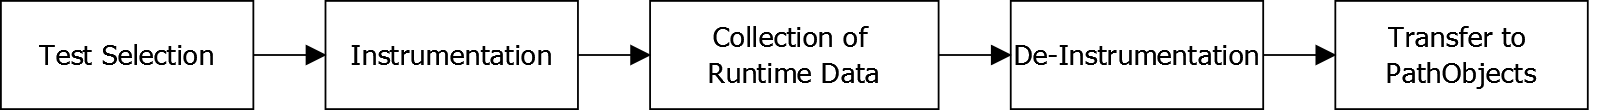
\includegraphics[width=0.9\textwidth]{../images/04-Tracing}
	\caption[TOC Caption]{Tracing foo}
	\label{fig:ImplementationTracing}
\end{figure}

Figure \ref{fig:ImplementationTracing} depicts the fundamental steps that are performed by the \textsc{PathTools} tracing framework to generate an execution trace.
First, the user selects a test case she wishes to analyze.
For instance, this can be done through the test coverage information

Method wrappers offer a convenient way to intercept the execution of specific methods.
As the name suggests, they wrap instances of \inlinecode{CompiledMethod} and take their place in the method dictionary of the corresponding class.
They can be utilized to execute code before and after the invocation of the wrapped method.
Furthermore, they allow the inspection and manipulation of arguments as well as of the return value of a message send.
Thereby, the operation of method wrappers is fully transparent for the callers of wrapped methods.

In order to be suitable for the purposes of \textsc{PathObjects}, the tracing framework had to be extended in two places.
First, a custom \inlinecode{MethodWrapper} had to be implemented that collects the information required for the reconstruction of object interactions.
For each wrapped executed method, this specialized wrapper reports integer identifiers of the receiving object, of the method arguments, and of the return value to the tracer.
Thereby, argument objects are flattened.
That means that if collections of objects are used as arguments, the identifiers of the objects contained in a collection are reported in addition to the identifier of the collection object itself.
Note that an identifier for the sender of a message is not captured, since it would require the expensive operation of stack inspection.
However, this information can be easily reconstructed from the tree structure of the traces, since the sender of a message is identical to the parent element of a call node in the call tree.

The second extension that had to be made is the implementation of a custom \inlinecode{Tracer} that provides some functionality required by our method wrappers and for additional refinement runs.
It provides an implementation of our object identification approach (cf. Section \ref{ss:ImplementationTracingIdentification}) that is used by the method wrappers to generate unique and stable identifiers for objects that occur during tracing.
Furthermore, it provides entry points for the exploration of outbound object references, and is responsible for the execution of refinement runs that are necessary to collect this information (cf. Section \ref{ss:ImplementationTracingReferences}).

\subsection{Reference Tracing}
\label{ss:ImplementationTracingReferences}

\section{Analyses}

\section{Visualization}
\subsection{Graph Layouting}
\subsection{Information Layers}